\documentclass[12pt,letterpaper]{article}
\usepackage{cite}
\usepackage{amsmath}
\usepackage{amsfonts}
\usepackage{array}
\usepackage{dsfont}
\usepackage{amssymb}
\usepackage{amsthm}
\usepackage{bbold}
\usepackage{fullpage}
\usepackage{mathtools}
\usepackage{enumitem}
\usepackage{mathrsfs}
\usepackage[margin=0.9 in]{geometry}
\usepackage{hyperref}
\usepackage{graphicx}
\usepackage{gensymb}
\usepackage{xcolor,colortbl}
\usepackage[format=plain,
labelfont={bf,it},
textfont={it}]{caption}
\usepackage{float}


\newcommand*{\SignatureAndDate}[1]{%
	\par\noindent\makebox[2.5in]{\hrulefill} \hfill\makebox[2.0in]{\hrulefill}%
	\par\noindent\makebox[2.5in][l]{#1}      \hfill\makebox[2.0in][l]{Date}%
}%
\newcolumntype{L}{>{\centering\arraybackslash}m{2cm}}
\newcolumntype{P}{>{\centering\arraybackslash}m{3cm}}
\newcolumntype{Q}{>{\centering\arraybackslash}m{4cm}}
\setlength{\parindent}{0em}

\allowdisplaybreaks

\newcommand{\R}{\mathds{R}}
\newcommand{\Z}{\mathds{Z}}
\newcommand{\Rplus}{\mathds{R}_{> 0}}
\newcommand{\Zplus}{\mathds{Z}_{\geq 0}}
\newcommand{\F}{\mathds{F}}
\newcommand{\N}{\mathds{N}}
\newcommand{\T}{\mathds{T}}
\newcommand{\s}{\mathds{S}}
\newcommand{\C}{\mathds{C}}
\newcommand{\CDFT}{\mathscr{F}_{CD}} %Fourier transform
\newcommand{\ip}[2]{\langle #1, #2\rangle}


\setlength{\parskip}{0.5em}


\makeatletter
\newsavebox\myboxA
\newsavebox\myboxB
\newlength\mylenA

\begin{document}
	
\section{Context and Motivation}

\subsection{Changing Cities}

By 2050, it is projected that 86 \% of the developed world will reside in urban areas \cite{Economist}. 
As a result of the adoption of the motorized vehicle, cities have become increasingly multi-centred, with retail parks and industrial estates far removed from the city centre \cite{SustainableTransport}. 
As a result of the changing layout of modern cities, traditional public transport has been rendered largely ineffective at efficiently transporting the population within the city \cite{SustainableTransport}. 
A British study showed that 83\% of commuting trips and 90\% of business trips in the country involved only a single passenger in a car \cite{NTS}, highlighting that the supply of mass, group transit do not meet the travel demands of modern society.
\\
\\
The lack of effective transportation infrastructure also has a considerable impact on the environment. 
The United States Environmental Protection Agency has determined that 14\% of global emissions are as a result of the transportation sector \cite{EPA}. 
Meanwhile, a Belgian case study showed that 47\% of trips and 54\% of distance travelled in that country was for the purpose of urban commuting \cite{Belgium}. 
Clearly, the environmental impact of urban transportation is considerable.

It has been determined that an effective transportation system for a modern city must satisfy the following constraints \cite{SustainableTransport}:

\begin{enumerate}
	\item is available on demand
	\item goes non-stop from start to destination
	\item is easily accessible and offers a full choice of destinations
	\item is strongly environmentally friendly
	\item is low cost
	\item has demonstrably high safety together with personal security
	\item integrates well with other forms of transport
\end{enumerate}

Personal electric transport (PET) has the potential to satisfy the transportation demands of a modern city. 
\subsection{The RipStik}
A caster board, known commercially as a RipStik, is a two-wheeled, human powered vehicle. 
The board is similar to a skateboard; however, it features two platforms, each with a wheel connected to an inclined free spinning caster. 
These platforms are connected by a torsion bar. 
This gives the caster board rider the unique ability to generate propulsion without removing their feet from the board through a series of small turns. 
This configuration also allows for tighter turning and more responsive speed control when compared to a skateboard. 
These characteristics could make the RipStik a practical vehicle for the urban commuter.
\begin{figure}[!htb]
	\centering
	\minipage{0.5\textwidth}
	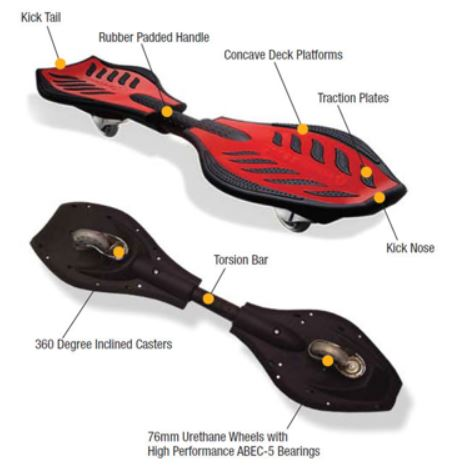
\includegraphics[width=\linewidth]{RipStik.JPG}
	\caption{Detailed description of the components of a RipStik \cite{PIC}}\label{fig:RipStik}
	\endminipage
\end{figure}
\par
A significant inhibitor to widespread RipStik adoption is developing competency in riding the board. 
As part of the RipStik’s design, a unique, full-body movement is required to generate the necessary forces for propulsion. 
For most new riders, this technique requires significant practice in order to develop the ability to ride a RipStik safely with confidence. 
Developing an electronic control system for the vehicle could facilitate riding, reducing the learning curve associated with the board while preserving the advantages of the RipStik. 
However, a RipStik is a sophisticated mechanical system and will require complex mathematical modelling to understand and represent all forces present in the system at a given time.

The addition of a control system to a caster board presents the potential for significant conflicts. 
Aside from the challenges associated with the development of the mathematical model and control system, issues pertaining to the patents for a caster board \cite{casterboardPatent} and restricted operation of the device \cite{TOLaws} may represent a barrier in bringing the product to market. 
Additionally, a mechanical system will be required to execute the commands of the control system. 
The difficulties associated with the recycling of batteries \cite{BatteryRecharge}, housing \cite{PlasticAssessment} and motors may threaten the environmental feasibility of the final design. 
The system may also be susceptible to "hacking" by outside sources \cite{DEFCON}, which could pose a significant safety risk to the operator. 
If these issues are addressed and mitigated, the potential of the device to minimize injuries associated with riding caster boards and to serve as a viable alternative to motor vehicles can be realized. 
This product has the potential to redefine urban commuting across the world by introducing a safe, cost-effective and environmentally-friendly option for short distance travel. 



\newpage
\bibliography{Bibliography}{}
\bibliographystyle{unsrt}

\end{document} 